\section{Problem 7}
Modeling expressions as fuzzy subsets in the context of fuzzy logic allows us to handle the uncertainty and imprecision inherent in certain descriptions like "large," "very small," or "medium-weight." In fuzzy logic, each element of the subset has a degree of membership ranging from 0 to 1, where 0 means "not a member at all" and 1 means "fully a member".\\
Below are examples of how you might model the given expressions as fuzzy subsets using MATLAB code snippets, assuming some reasonable definitions for each term.\\

\underline{LARGE INTEGERS}\\
For "Large integers," we need a membership function that gradually increases as the integers become larger. A simple way to model this is to use a function that increases the membership score as the number exceeds a certain threshold. However, defining "large" is subjective and can vary depending on the context. For simplicity, let's assume integers greater than 100 are considered large, but the transition starts at 50, becoming more "large" as the number increases.

\begin{figure}[h]
	\centering
	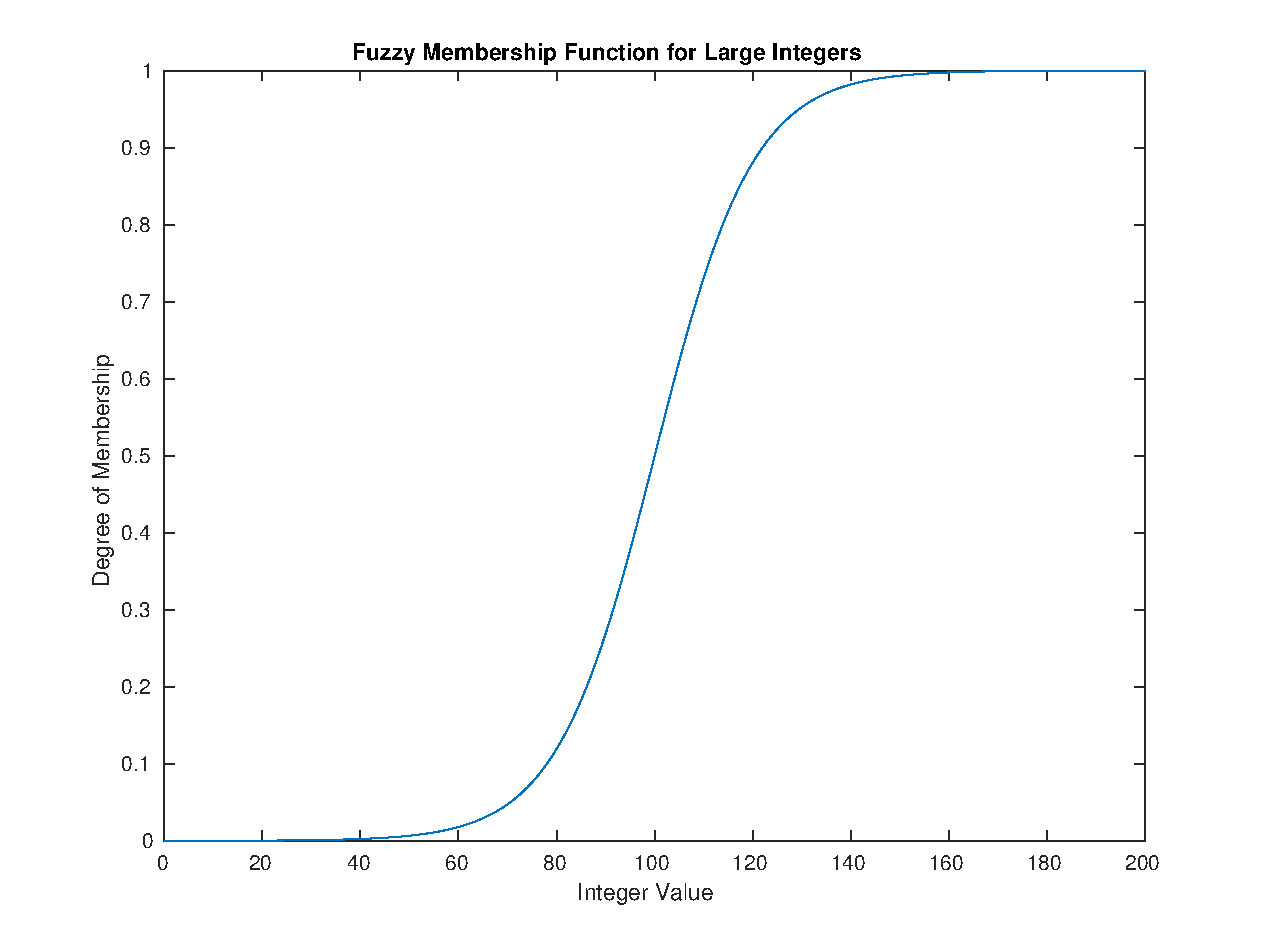
\includegraphics[width=0.6\textwidth]{../Problem 7/large_int.pdf}
	\caption{Fuzzy membership function for Large Integers}	
\end{figure}
we are using the sigmoid function for a smooth transition.
\vspace{5mm}

\underline{VERY SMALL NUMBERS}\\
For "very small numbers," we can consider numbers close to zero as having a higher degree of membership. "Very small numbers" can include both positive numbers close to zero and negative numbers. For this, a membership function that assigns higher scores to numbers closer to zero can be used. We'll focus on positive numbers for simplicity, but this can be adjusted to include negatives.

\begin{figure}[H]
	\centering
	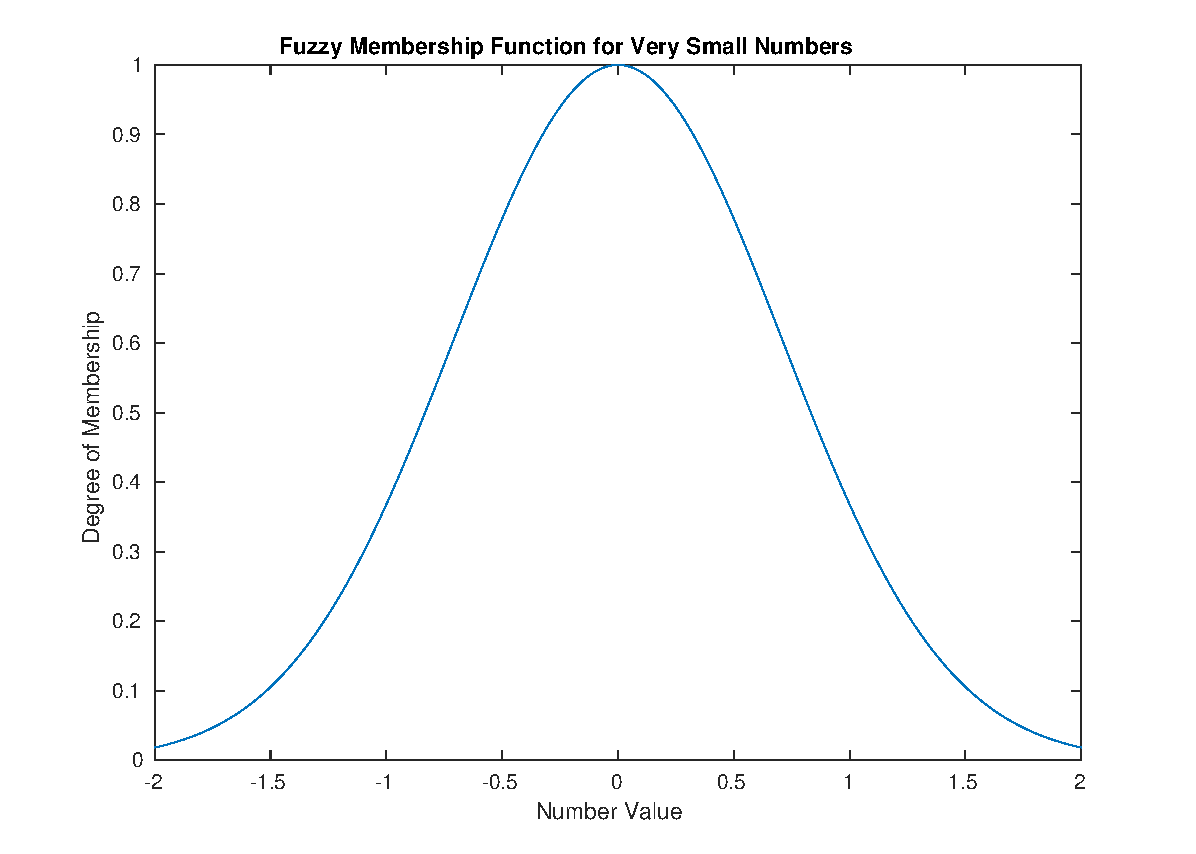
\includegraphics[width=0.6\textwidth]{../Problem 7/small_int.pdf}
	\caption{Fuzzy membership function for Very Small Numbers}	
\end{figure}
we are using the Gaussian function centered at 0.
\vspace{5mm}

\underline{MEDIUM-WEIGHT MEN}\\
Assuming the average weight range for medium-weight men is between 70kg and 90kg, with the peak at 80kg, we can define a triangular membership function.
